% !TeX root = ../thuthesis-example.tex

\chapter{评价指标与实验结果}

本章首先介绍本文所实现的多摄像头多目标行人位置估计算法中所采用的实验评价指标,然后详细阐述实验过程和实验的环境、参数。最后,将实验结果与目前业界最新算法进行比较,并提出未来可能的改进建议。

\section{评价指标}

精确率(Precision)和召回率(Recall)是信息检索和统计学分类领域的两个应用很广泛的度量,用来评价结果的质量。本文采用了精确率、召回率来衡量最终位置估计效果。然而,由于在大规模数据集合中,精确率和召回率两个指标往往是相互制约的,因此,本文还采用了F分数(F-score)来综合权衡精确率和召回率。即,本文共使用了精确率、召回率和F分数三个评价指标来衡量最终的位置估计效果。

为了得到上述三个评价指标,首先需要得到实验结果的混淆矩阵(Confusion Matrix)。混淆矩阵也称误差矩阵,在本文中为两行两列的矩阵形式,其主要参数有四个,即真阳性(True Positives, TP)、真阴性(True Negatives, TN)、假阳性(False Positives, FP)、假阴性(False Negatives, FN)。在本文实验中,TP集合为与实际位置相符的预测点;TN集合应为预测点之外的点中排除实际位置的点,由于计算上述三个评价指标并没有用到TN集合,故被忽略;FP集合为预测点中没有命中实际位置的点;FN集合为没有被预测到的实际位置点。在本实验中,预测点与实际位置命中的判定半径为$r=0.5m$,即若预测点与实际点距离相聚小于50cm即判定为成功估计了行人的位置。

上文提到,计算混淆矩阵的参数时,需要判定预测点与实际位置点是否对应,从而判定是否正确预测。现在,我们得到了对行人位置在地面上的最终预测点,同时,我们有行人地面实际位置的标注,那么就需要将这些预测点和实际标注一一匹配起来,从而可以计算预测点与实际点之间的距离,以判断是否预测成功。解决上述匹配问题的方法可以抽象为图论中寻找最大匹配的算法,在本文中,上述问题抽象为在二分图中寻找最大匹配。因此,我们实现了匈牙利算法(Hungarian Algorithm)来解决这一问题。匈牙利算法利用深度优先搜索来不断寻找增广路。它从每个未匹配的实际地面点开始,如果直接找到了预测点中未匹配的点,则直接返回此匹配路径;若找到预测点已匹配的点,那么从该点匹配的点出发继续深度优先搜索未匹配点。

得到混淆矩阵后,可以计算上述三个评价指标。
\begin{itemize}
    \item 精确率(Precision) 精确率是针对预测结果而言的,它表示的是预测点中有多少是预测正确的。精确率显示了模型预测点的精确性,可由下式计算:
        \begin{equation}
            \text{Precision}=\frac{\text{TP}}{\text{TP}+\text{FP}}
        \end{equation}
    \item 召回率(Recall) 召回率是针对原来的样本而言的,它表示的是实际位置点中有多少被预测命中了。召回率显示了模型是否能够估计出视野中更多行人的实际位置,其可由下式计算:
    \begin{equation}
        \text{Recall}=\frac{\text{TP}}{\text{TP}+\text{FN}}
    \end{equation}
    \item F分数(F-score) 精确率和召回率指标有时候会出现矛盾的情况,这样就需要综合考虑二者,最常见的方法就是利用F分数,即精确率和召回率的加权调和平均:
    \begin{equation}
        \text{F-score}=(1+\beta^2)\cdot \frac{\text{Precision} \cdot \text{Recall}}{\beta^2 \cdot \text{Precision} \cdot \text{Recall}}
    \end{equation}
    本文中令$\beta=1$,即实际上使用F1-score。
\end{itemize}

\section{实验设置和结果分析}

首先,进行层次聚类数据融合的实验,以生成后续神经网络输入的热图。为了得到最优的二维高斯概率分布热图,需要对前述生成二维高斯概率分布的超参数进行调整。实验过程是,在合理的范围内取超参数得到层次聚类结果,然后利用精确率、召回率和F分数三个评价指标来反向优化,即适当改变超参数的值,直到F分数达到最大,此时得到的超参数即为最优超参数。

调整参数的过程中,可以发现,当高斯概率形状调整参数$k\rightarrow1$,则二维高斯概率趋于扁平,长轴方向为$\bm{v}$,若$k\rightarrow0$,则二维高斯概率趋于扁平,长轴方向为$\bm{v}'$,若$k\rightarrow0.5$,则二维高斯概率趋于一个圆形。在实际聚类过程中,二维高斯概率分布的形状既不能太过扁平也不能太过圆滑,在实验中,可得当$k=0.85$时,F分数最高。而二维高斯概率分布中的$k_c$描述了二维高斯概率分布覆盖范围的大小,在实验中可以得到当$k_c$接近于700时,聚类效果最好。聚类的阈值距离$t_g$在趋于0时,同一行人在不同摄像机中得到的二维高斯概率分布难以聚为同一类,而若趋于一个较大值时,会导致不同行人的聚类和错误的聚类,在实验中,可以得到$t_g$在19cm附近时,F分数会取得最大值。脚踝节点的保留阈值$t_{ankle}$的作用是抑制AlphaPose中得到的置信度过低的姿态节点,在实验中可以发现,保留置信概率大于0.35的脚踝节点可以达到最佳的聚类效果。最终经过实验调优,可得到最优的超参数如下表~\ref{parameter_table}所示。利用此最优超参数生成后续神经网络输入的热图,可以最大化神经网络方法的效果。
\begin{table}
    \centering
    \caption{反向优化得到的最优超参数}
    \begin{tabular}{lll}
        \toprule
        参数 & 值  & 描述         \\
        \midrule
        $k_{c}$ & 700 & 二维高斯概率分布中$C=k_{c}\bm{v}^\top\bm{v}, C'=k_{c}\bm{v}'^\top\bm{v}'$中的$k_{c}$ \\
        $k$   & 0.85 &  二维高斯概率分布中$\Sigma=kC + (1-k)C'$中的$k$   \\
        $t_{g}$ & 19cm &  层次聚类中聚为一类的阈值距离  \\
        $t_{ankle}$ & 0.35 &  单目探测器结果中保留概率超过$t_{ankle}$的脚踝节点 \\
        \bottomrule
    \end{tabular}
    \label{parameter_table}
\end{table}

以上述超参数的设置,得到的层次聚类结果如图~\ref{HC_a}所示,其中黄色三角形为行人实际地面位置,而橙色星形为层次聚类得到的行人地面位置估计。作为补充,图~\ref{HC_b}中也显示了作为层次聚类输入的人物位置二维高斯概率分布(以椭圆形表示),其中来自同一摄像头的分布用同一种颜色表示,同一颜色、同一序号的二维高斯概率分布为同一聚类。
\begin{figure}
    \centering
    \subcaptionbox{\label{HC_a}}
      {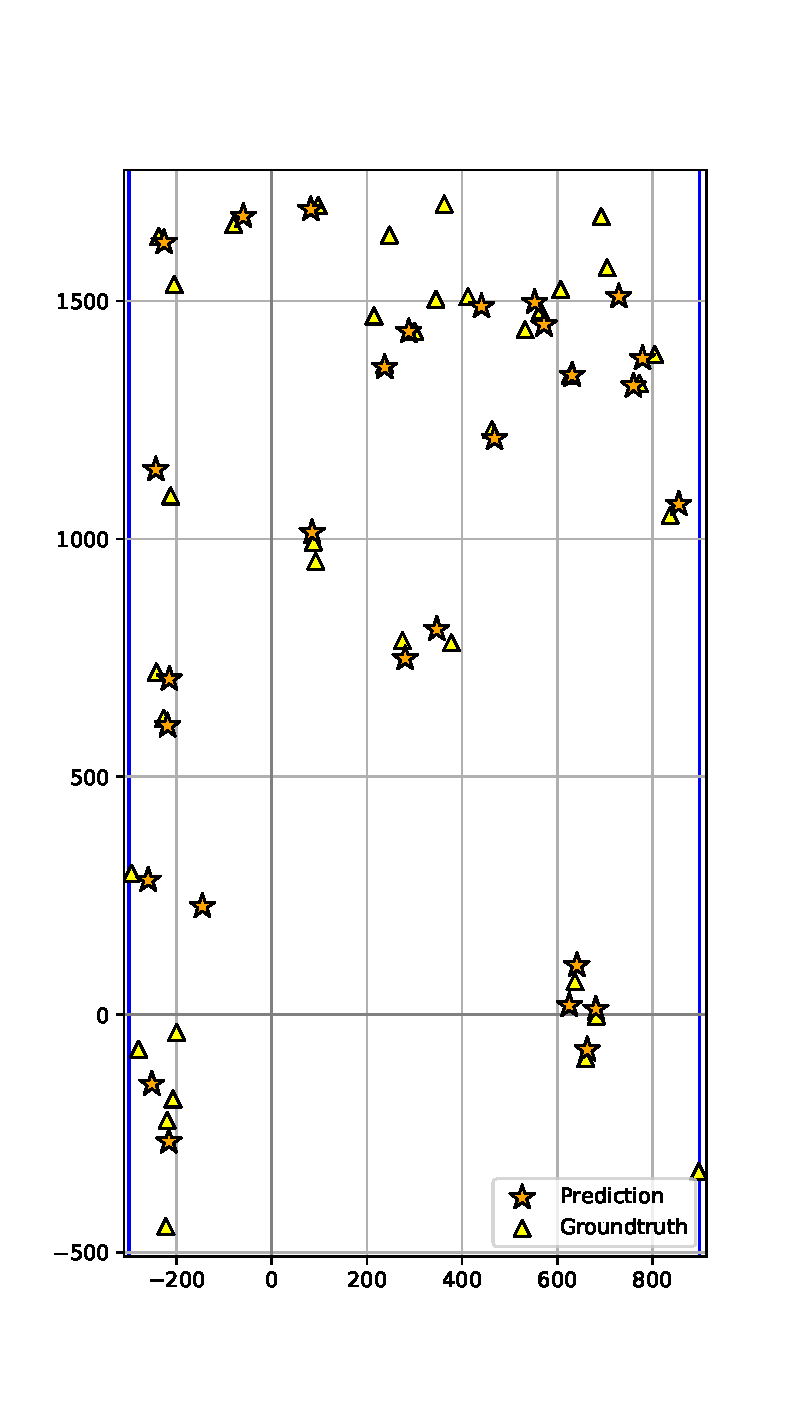
\includegraphics[width=0.4\linewidth]{HC.pdf}}
    \subcaptionbox{\label{HC_b}}
      {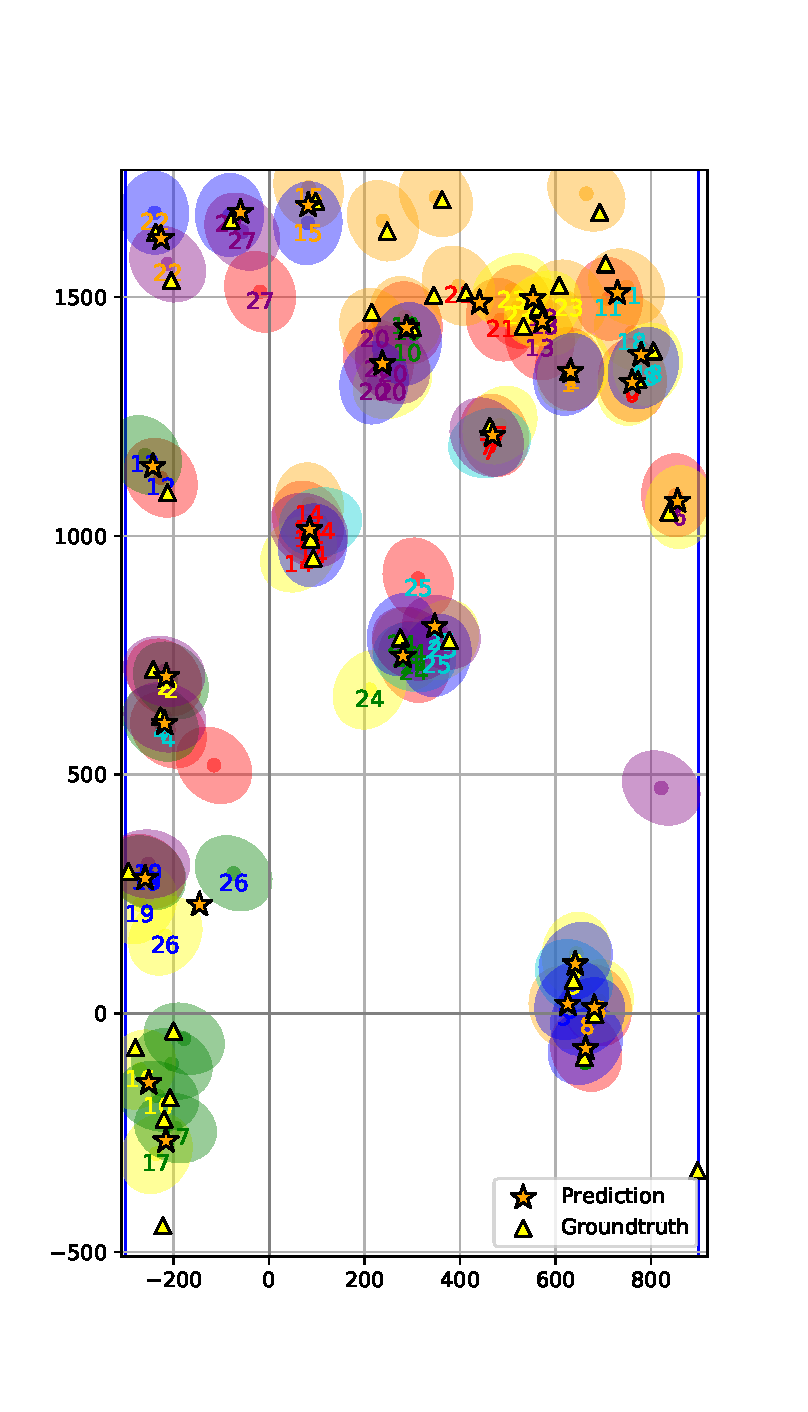
\includegraphics[width=0.4\linewidth]{HC_gaussian.pdf}}
    \caption{层次聚类结果}
    \label{HC}
\end{figure}

利用表~\ref{parameter_table}中的超参数进行层次聚类的数据融合之后,可以初步得到行人位置估计结果,这些实验结果与深度学习方法的比较如表~\ref{experiments}所示。

在深度学习方法中,主要在WildTrack数据集上进行实验。其中,作为训练集的是从WildTrack数据集提供的七个摄像头视频提取到的视频帧,每个摄像头共有11558张图片,其中真值由官方提供的400张图片真值插值得到;作为测试集的是WildTrack数据集提供的每个摄像头400张的去畸变图,提供了真值标注。实现的ResUNet和ResUNet++网络均基于PyTorch,部署在NVIDIA RTX 3090 GPU进行训练,系统版本为Ubuntu 18.04,提供CUDA 11.3支持。在训练的过程中,输入热图和输出预测图的尺寸均为$224\times 672$,输入网络时采用的Batch Size为4,使用Adam优化器进行调优。同时,为了避免网络难以收敛到最优状态,初始学习率设置为1e-3,每20个训练周期(epoch)学习率衰减为原来的0.1倍,一共训练100个周期。

将深度学习方法中ResUNet和ResUNet++网络的实验结果与目前领域内几个深度学习方法的比较如下表~\ref{experiments}所示。
\begin{table}
    \centering
    \caption{层次聚类方法、ResUNet和ResUNet++与其他方法实验效果比较}
    \begin{tabular}{llll}
        \toprule
        方法 & 精确率  & 召回率 & F分数                       \\
        \midrule
        Deep-Occlusion\cite{baque2017deep} & 95\% & 80\% & 86\%                  \\
        Generalized Mutiview Detection\cite{vora2021bringing} & 94\% & 93\% & 93\%  \\
        Hierarchical Clustering & 87\% & 62\% & 72\%         \\
        ResUNet & 92\% & 70\% & 79\%                         \\
        ResUNet++ & 95\% & 85\% & 90\%                      \\
        \bottomrule
    \end{tabular}
    \label{experiments}
\end{table}

由表~\ref{experiments}可以看出,ResUNet++网络结构效果比ResUNet效果好很多,而没有使用神经网络的层次聚类融合方法效果最差。同时,也可以发现,ResUNet++在多摄像头多目标行人位置估计领域,在未使用行人重识别和时序信息的情况下,达到了接近目前业界领先算法的效果。然而,我们可以发现几乎所有的结果中精确率都比召回率更高,尤其是ResUNet得到的结果。这是因为网络对输入的热图进行特征提取时,那些遮挡较少、有多个摄像头同时拍摄的行人会在热图中生成明显的概率分布聚集,从而提高了预测点的精确率。然而,在人员密集的区域,对行人的检测和估计难度迅速增大,从而导致了很多遮挡行人难以被检测到,因此导致预测点比实际点数量更少,从而降低了召回率。在本文提出的多摄像头行人位置估计算法中,关键的困难不是预测得到的位置点与实际点距离偏离过大,而是对于遮挡严重的行人,即使检测到其存在,也很难在多个摄像头中同时生成其二维高斯概率分布,导致生成的热图中遮挡严重的行人的特征比较混乱,因此容易被网络忽略和误判。因此,预测点将会比实际点少,从而导致召回率降低。

\begin{figure}[H]
    \centering
      \subcaptionbox{输入热图\label{300heatmap}}
      {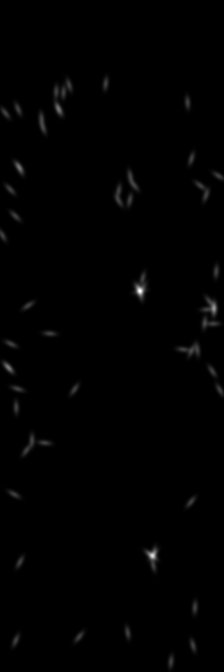
\includegraphics[width=0.2\linewidth]{000300_inputs.png}}
      \subcaptionbox{真值标签\label{300label}}
      {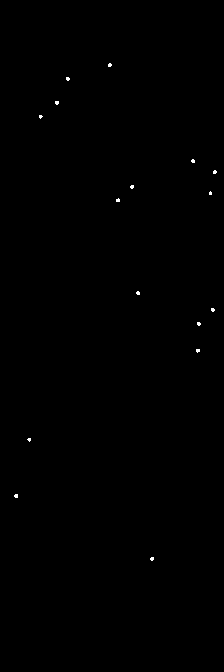
\includegraphics[width=0.2\linewidth]{000300_label.png}}
      \subcaptionbox{ResUNet++\label{300RPP}}
      {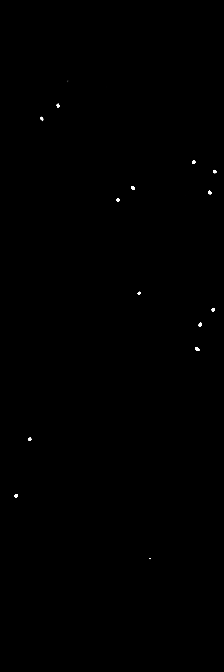
\includegraphics[width=0.2\linewidth]{000300_RPP.png}}
      \subcaptionbox{ResUNet\label{300R}}
      {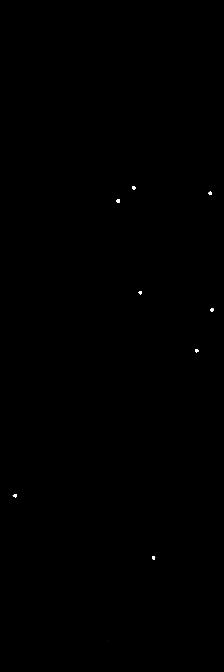
\includegraphics[width=0.2\linewidth]{000300_R.png}}
    \caption{预测结果示例1}
    \label{success}
\end{figure}
接下来,结合具体例子对估计结果进行分析。图~\ref{success}展示了一个位置估计相对比较成功的结果,在这一帧中,ResUNet++得到的结果精确度达到了100\%,召回率为94\%,F分数为97\%,而ResUNet得到的结果为精确度100\%,召回率为50\%,F分数为67\%。其中,预测比较成功的原因主要是当前图片内人物数量不多,互相遮挡的情况比较少,因而在第一步的AlphaPose姿态节点检测中就能得到比较准确的结果,得到的二维高斯概率分布图和生成的热图比较简单,同时,由于网络结构比较深入,对于这种相对简单的场景能够比较容易抓取其概率分布的特征,因此在ResUNet和ResUNet++中都取得了相对不错的效果。

\begin{figure}[H]
    \centering
      \subcaptionbox{输入热图\label{045heatmap}}
      {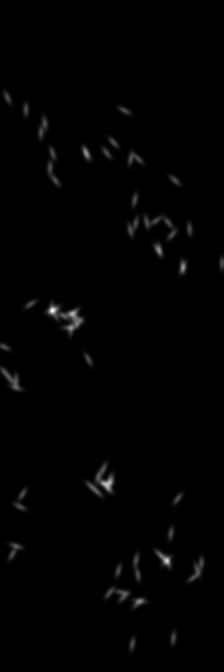
\includegraphics[width=0.2\linewidth]{000045_inputs.png}}
      \subcaptionbox{真值标签\label{045label}}
      {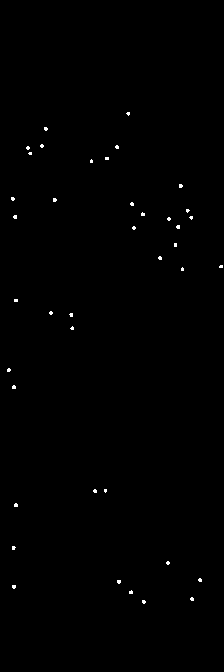
\includegraphics[width=0.2\linewidth]{000045_label.png}}
      \subcaptionbox{ResUNet++\label{045RPP}}
      {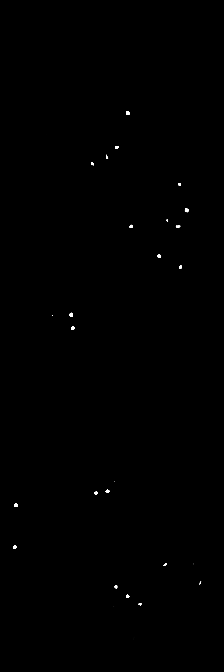
\includegraphics[width=0.2\linewidth]{000045_RPP.png}}
      \subcaptionbox{ResUNet\label{045R}}
      {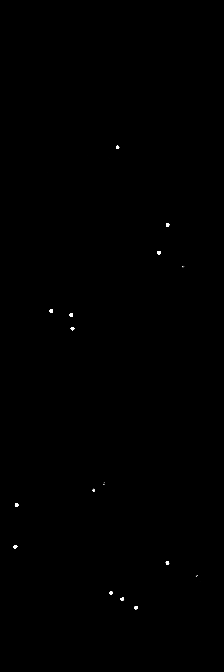
\includegraphics[width=0.2\linewidth]{000045_R.png}}
    \caption{预测结果示例2}
    \label{failure1}
\end{figure}
然而,在图~\ref{failure1}中,可以看出预测的结果并不十分理想。在这一帧中,ResUNet++得到的精确度为92\%,召回率为58\%,F分数为71\%,而ResUNet为精确度为77\%,召回率为33\%,F分数为46\%,可见这一帧的预测过程中出现了很大障碍。从精确度和召回率相差很大的现象可以得出,在这一帧中最大的问题是有很多行人没有判断出来。出现这种现象是因为所采用的AlphaPose单目检测器,并不能直接输入高清图片,而是只能输入尺寸非常小的$256\times 192$的图片,在压缩尺寸的过程中自然丢弃了很多图像的内容信息。从图~\ref{failure1}中可以看到,ResUNet与ResUNet++都在左侧边缘区域以及左上角距离摄像头比较远的区域出现了很多未探测到行人的状况,印证了上述AlphaPose输入尺寸过小,导致较远处行人分辨率过低,难以辨认姿态节点,即使得到节点,其准确性也很差。针对此问题,未来可以将姿态估计部分改为输入高清图片,探测到行人后截取其检测框,然后将检测框输入网络判断姿态,便可完全利用摄像头捕捉到的行人外表信息,而不是现在将整幅图直接压缩尺寸后输入,造成信息损失。此外,在图中上侧的行人密集处,也出现了预测不全,这是因为此帧中行人密集处在不同摄像机视角下都有较多的遮挡,在这种复杂遮挡的背景下,不仅仅AlphaPose得到的姿态不准确,而且生成的二维高斯概率分布图也呈现出一种混乱的状况。针对这一问题,需要改进二维高斯概率分布建模过程。未来可以给每个二维高斯概率分布加入与摄像头距离相关的权重,或者让与摄像头的距离成为调节二维高斯概率分布大小和形状的重要因素,这样,可以将摄像头远近不同产生不同置信概率的信息加入到位置概率建模和热图生成过程中,如此可减少远处行人的概率分布混乱问题,同时增强近处行人的估计准确度。最后,左侧行人位置的估计不全还可能是因为左侧区域有一些行人在区域的边缘处,于是数据集的标注会呈现一定的不确定性,此外,此区域还有一些坐在台阶上的行人,这些行人在AlphaPose的探测中常常会被错误探测,从而造成了最终预测结果的失误。

\begin{figure}[H]
    \centering
      \subcaptionbox{输入热图\label{015heatmap}}
      {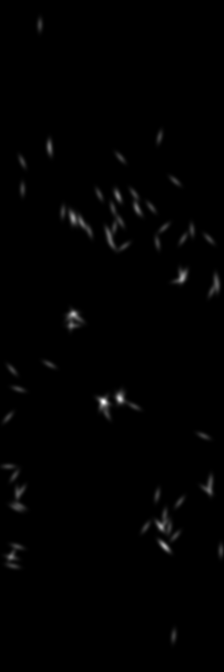
\includegraphics[width=0.2\linewidth]{000015_inputs.png}}
      \subcaptionbox{真值标签\label{015label}}
      {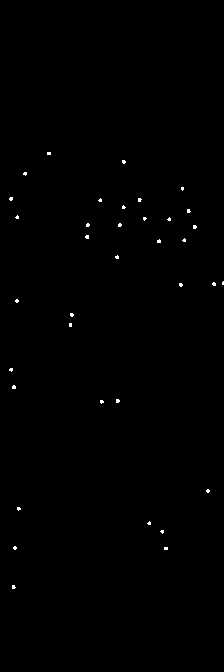
\includegraphics[width=0.2\linewidth]{000015_label.png}}
      \subcaptionbox{ResUNet++\label{015RPP}}
      {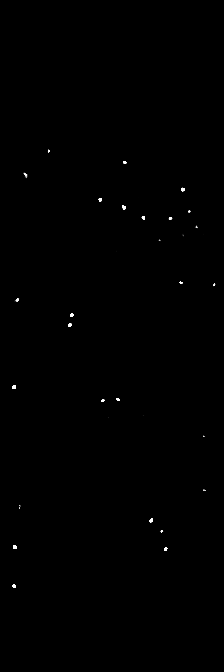
\includegraphics[width=0.2\linewidth]{000015_RPP.png}}
      \subcaptionbox{ResUNet\label{015R}}
      {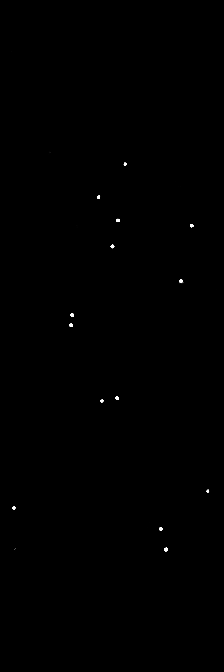
\includegraphics[width=0.2\linewidth]{000015_R.png}}
    \caption{预测结果示例3}
    \label{failure2}
\end{figure}
此外,在图~\ref{failure2}中,效果也不太理想,同时ResUNet++和ResUNet所得到的结果有较大的差异。在这一帧中,ResUNet++得到的精确度为97\%,召回率为75\%,F分数为84\%,而ResUNet为精确度为93\%,召回率为39\%,F分数为55\%。可见ResUNet的结果召回率相当低。在图中对比也可以发现,ResUNet++在人群密集区域有较多的未命中点,而ResUNet预测结果中有很多真实位置没有被估计到。ResUNet++在人群密集区域的缺陷上文已经举例分析,因此此处分析ResUNet与ResUNet++预测结果的差异。对比可见,在输入热图大块特征比较明显,即有多个摄像头同时拍摄到同一个行人的情况下,ResUNet++和ResUNet都呈现了不错的效果。但是在高斯概率分布相对混乱的区域,或者说,局部特征和纹理比较复杂的区域,ResUNet++取得了比ResUNet好得多的效果。这是因为ResUNet++加入的挤压和激励单元提高了网络对局部特征的敏感性,抑制了不必要的一些混乱的特征,同时空洞空间金字塔池化和注意力机制使得网络可以控制视野,专注于重要的局部特征,显著提升了特征的质量。因此ResUNet++相比ResUNet在概率分布比较混乱的部分能够取得更准确的结果。

最后,在层次聚类的反向调优过程中,可以通过设计更好的调优方法找到最佳的参数,从而得到更准确合理的热图,提高网络输出效果。此外,在将网络输出的预测图转变为实际位置时,也会产生一些误差,这些误差会对最终结果造成一定影响。

\section{本章小结}

本章中主要介绍了实验的评价指标、实验设置细节和具体实验结果的分析。实验的评价指标主要使用了精确率、召回率和F分数三个指标来衡量算法位置估计的效果,实验设置上,对数据集进行扩充以增加训练量,同时利用学习率衰减的训练策略,提升了训练效果。在实验结果方面,仅仅使用层次聚类来得到行人的位置估计的算法效果并不好,而在层次聚类的基础上利用ResUNet和ResUNet++的深度学习网络可以达到较好的效果。最后对实验结果进行分析,同时提出了一些未来改进的方向。所实现的ResUNet++在ResUNet基础上改进而来,达到了接近目前最优算法的性能。